\section{Polynomial and Calculations}

For the polynomial:
\[
y = 2x^3 - 3x^2 + x - 5
\]

We calculate \( y \) for the given values of \( x \):

\begin{table}[t]
\centering
\begin{tabular}{|c|c|}
\hline
\textbf{x} & \textbf{y} \\
\hline
-2 & -35 \\
-1 & -11 \\
0 & -5 \\
1 & -5 \\
2 & 1 \\
\hline
\end{tabular}
\caption{Values of \( y \) for the polynomial \( y = 2x^3 - 3x^2 + x - 5 \)}
\end{table}

Below is the plot of the polynomial and the given points:

\begin{figure}[t]
\centering
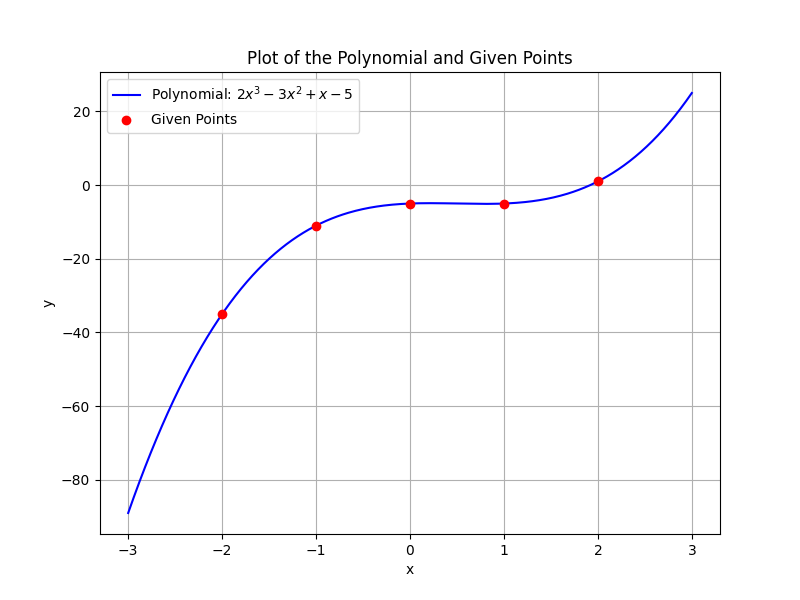
\includegraphics[width=0.8\textwidth]{PART3/1_polynomials/table1_1.png}
\caption{Plot of the polynomial $y = 2x^3 - 3x^2 + x - 5$ with given points.}
\end{figure}